\documentclass[12pt, a4paper]{article}
\usepackage{times}
\usepackage[magyar]{babel}
\usepackage{amsmath}
\usepackage[lmargin = 2.5 cm, tmargin = 2.5 cm, bmargin = 2.5 cm, rmargin = 2.5 cm]{geometry}
\usepackage{t1enc}
\usepackage{fancyhdr}
\usepackage{hyperref}
\usepackage{tabularx}
\usepackage{amsthm}
\usepackage{amssymb}
\usepackage{amsfonts}
\usepackage[usenames,dvipsnames]{xcolor}
\usepackage{float}
\usepackage{graphicx}
\usepackage{listings}
\usepackage{caption}
\usepackage{matlab-prettifier}
\usepackage{varwidth}
\usepackage{setspace}
\usepackage[style=ieee, citestyle=numeric-comp]{biblatex}
\usepackage{csquotes}
\usepackage{multicol}

\addbibresource{irodalomjegyzek.bib}

\begin{document}

\begin{center}
\LARGE\textbf{Hátoldali reflexiós echelon terahertzes forrás optimalizálása numerikus számításokon keresztül}\vspace*{0.7cm}\\\large
Illés Gergő $^{1,*}$, Krizsán Gergő $^{1,2}$, Pálfalvi László $^1$, Tibai Zoltán $^1$, Almási Gábor $^1$, Hebling János $^{1,2,3}$, Tóth György $^1$\vspace*{0.4cm}\\\normalsize
\textit{$^1$ Pécsi Tudományegyetem, Fizikai Intézet, Pécs, Magyarország\\
$^2$ Szentágothai János Kutatóközpont, Pécs, Magyarország\\
$^3$ ELKH-PTE ?Nagy Térerősségű Terahertzes Kutatócsoport?, Pécs, Magyarország\\
$^*$ illesg@gamma.ttk.pte.hu}
\end{center}\vspace*{0.5cm}
\begin{abstract}\noindent
Az optikai terahertzes források fejlődésével lehetőség nyílt arra, hogy 1 mJ nagyságrendű impulzusenergiákat állítsunk elő \cite{wu20201}. Ezt az impulzusenergiát a döntött impulzusfrontú gerjesztés módszerét \cite{hebling2002velocity} használva sikerült elérni. Azonban a döntött impulzusfrontú gerjesztés módszerének számos korlátozó tényezője van. Az első, hogy a kristály nagy ékszöggel rendelkezik, a második, hogy a nagy impulzusfront-döntés következtében a pumpaimpulzus nagymértékű szögdiszperzióval rendelkezik, a harmadik pedig, hogy az elrendezésben használt leképző rendszer nem tökéletes, leképzési hibák keletkeznek. Ezen hibák enyhítésére lehetőséget ad a hátoldali reflexiós elrendezés \cite{krizsan2020lithium,toth2019single}. A Pécsi Terahertzes kutatócsoport már végzett számításokat az elrendezésen, azonban az akkor használt modell nem vette figyelembe a terahertzes impulzus visszahatását a pumpaimpulzusra.
\end{abstract}
\onehalfspace
\section{Az elrendezés vázlata}
A hátoldali reflexiós echelon elrendezés sematikus ábráját az 1. ábra mutatja be.
\begin{figure}[H]
\centering
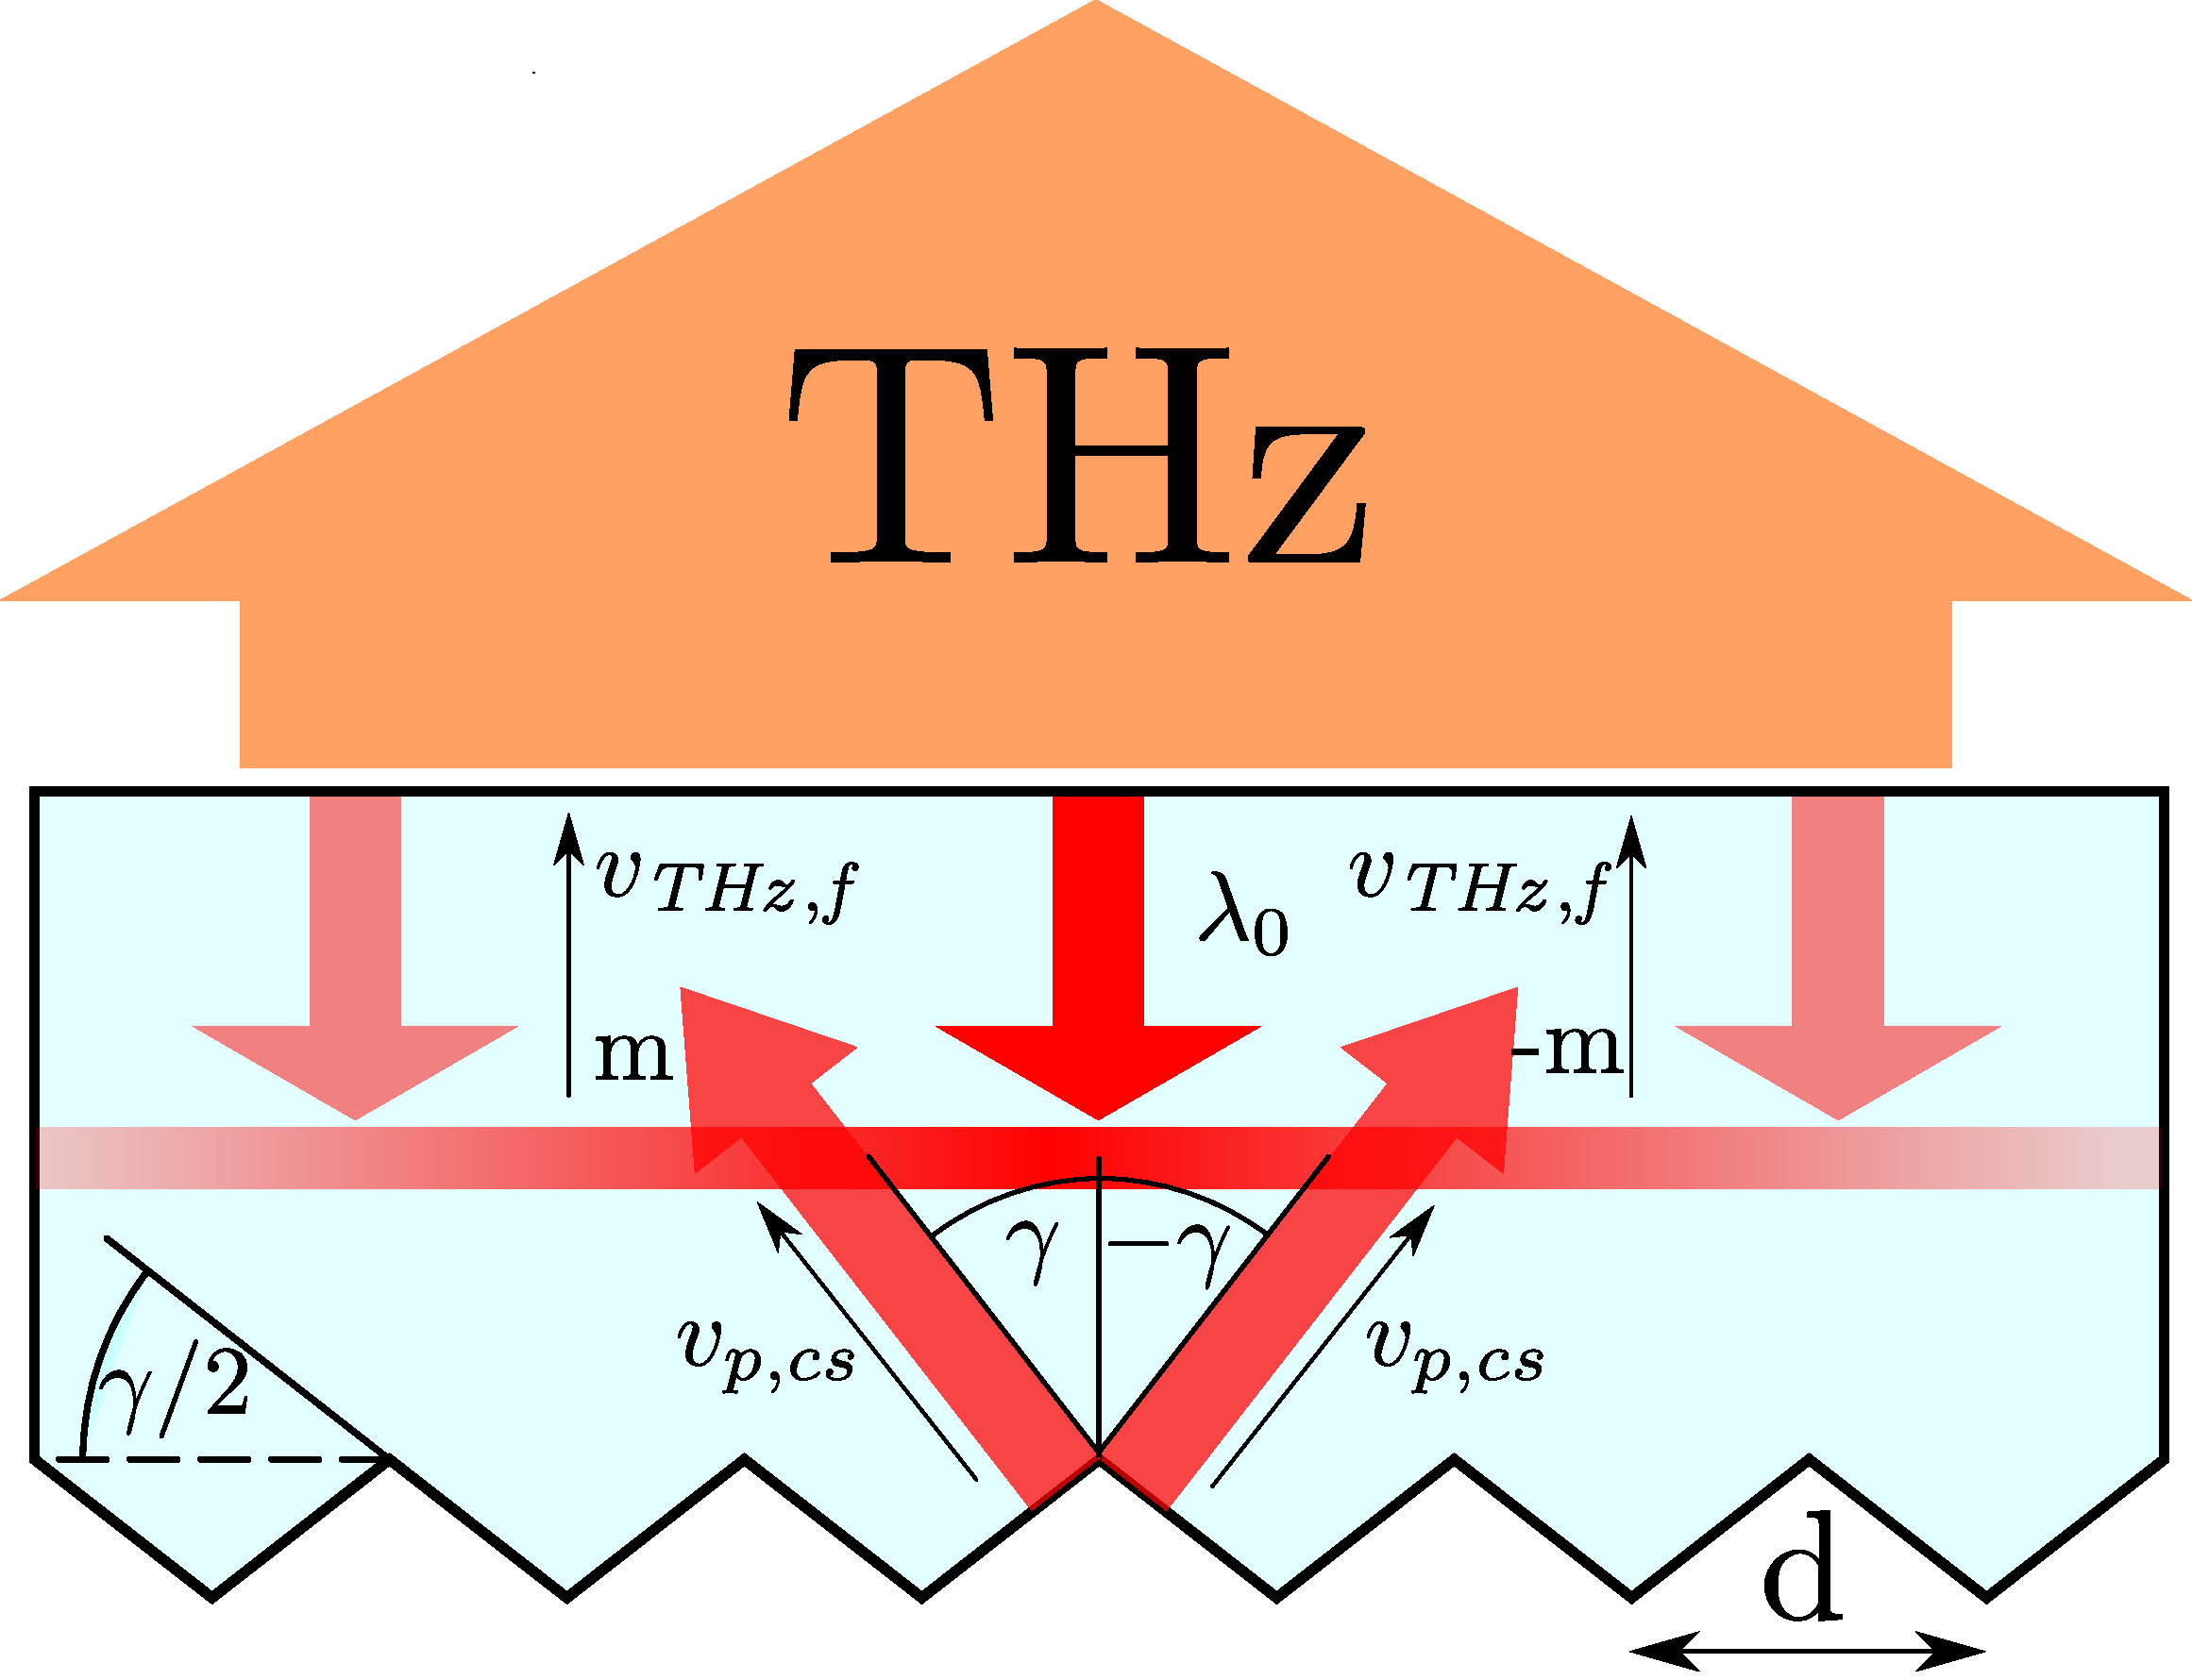
\includegraphics[width=0.7\textwidth]{rajz-1.pdf}
\caption{A hátoldali reflexiós echelon sematikus ábrája \cite{toth2019single}}
\end{figure}
Az elrendezés úgy működik, hogy a pumpaimpulzus a kristályra merőlegesen lép be, majd a kristály hátoldalához érve, a megmunkált felületen diffraktálódik. Ezen megmunkálásnak olyannak kell lennie, diffrakció következtében a kialakuló impulzusfrontdöntés megfeleljen a sebességillesztési feltételnek \cite{hebling2002velocity}. Amennyiben ez teljesül úgy hatékonyan fog keletkezni a terahertzes (továbbiakban THz-es) impulzus. Az keletkező THz-es impulzus a kristály belépő felületén fog távozni, haladási iránya pedig merőleges lesz erre a felületre, aminek következtében nagy hatásfokú lesz a kicsatolás. 
\section{Numerikus modell}
A számítások olyan numerikus modellel készültek amelyek figyelembe veszik a THz-es impulzus visszahatását a pumpaimpulzusra \cite{ravi2014limitations}. A döntött impulzusfrontú gerjesztési technika modellezésénél azt tapasztaltuk, hogy a visszahatás következtében nagy mértékben csökken az elérhető maximális térerősséget, valamint azt, hogy azon kristályhossz ahol a hatásfok maximális rövidebb lesz. További számolások során megállapítottuk, hogy a maximális hatásfokhoz tartozó kristályhosszt túllépve a THz-es impulzus megszűnik egyciklusúnak, a térerősségének maximuma nagymértékben csökken és ezáltal használhatatlanná válik. Az itt bemutatott eredményeket a \cite{ravi2014limitations}-ben bemutatott modell módosított változatával kaptuk.
\section{Eredmények}
\subsection*{Hatásfok}
Először vizsgáljuk az echelon elrendezés hatásfokát a döntött impulzusfrontú gerjesztés (továbbiakban TPF) elrendezés hatásfokával összehasonlítva. A számításokat 1030 nm-es központi hullámhosszú, 200 fs-os pumpaimpulzust feltételezve végeztük. Az eredményeket a 2. ábra mutatja.
\begin{figure}[H]
\centering
\includegraphics[width = 0.7\textwidth]{Origin/graph1.pdf}
\caption{A TPF és az echelon elrendezés hatásfoka}
\end{figure}
Az ábrán látható, hogy amíg a TPF elrendezés hatásfoka 2\% 0,5 mm-es kristályhossz esetén, addig a reflexiós echelon hatásfoka akér az 5\%-ot is elérheti 6 mm-es kristályhossz esetén. Ezen számítás alapján azt mondhatjuk, hogy az echelon elrendezés a kedvezőbb, azonban a hatásfok nem az egyetlen tényező. THz generálásnál fontos ezen felül az impulzus időbeli lefutása is, ezért vizsgáljuk meg a THz-es impulzus időbeli lefutását. Láthatjuk továbbá, hogy a TPF hatásfoka gyorsabban növekszik és egy egyértelmű maximumot vesz fel. Az echelon elrendezés hatásfoka a vizsgált tartományon folyamatosan növekszik.
\section*{A térerősségek időbeli lefutása}
A TPF elrendezésen végzett korábbi számításokból tudjuk, hogy az elrendezés akkor produkálja a legjobb minőségű THz-es impulzust amikor a maximális hatásfokhoz tartozó kristályhosszat használjuk. Továbbá azt is megállapítottuk szisztematikus számításokon keresztül, hogy amennyiben ennél nagyobb kristályhosszat használunk a THz-es impulzusban sok optikai ciklus jelenik meg, a csúcstérerősség pedig nagy mértékben lecsökken Ha kisebb kristályhosszakat vizsgálunk ott a THz-es impulzus közel egyciklusú, a maximális térerősség pedig alacsonyabb, mint a maximális hatásfokhoz tartozó kristályhossz esetén. Ezen okokból kifolyólag a TPF esetén a maximális hatásfokhoz tartozó kristályhossznál vizsgáljuk a THz-es impulzus időbeli alakját. Az eredményeket a 3. ábra mutatja.
\begin{figure}[H]
\centering
\includegraphics[width = 0.7\textwidth]{Origin/graph2.pdf}
\caption{A TPF és az echelon által keltett THz-es impulzus}
\end{figure}
Láthatjuk, hogy a két impulzus több szempontból is különbözik egymástól. A TPF által keltett impulzus egynél több optikai ciklust is tartalmaz, míg az echelon által keltett impulzus csak egyet. A másik különbség pedig a maximális térerősség. Ezen beállítások mellet a TPF elrendezéssel elérhető maximális térerősség 320 $\frac{KV}{cm}$ az echelon esetében pedig 500 $\frac{KV}{cm}$.
\section*{Következtetés}
A bemutattak alapján az mondhatjuk, hogy a hátoldali reflexiós echelon elrendezés ígéretes THz-es forrás. Számításaink azt mutatják, hogy az eddig leggyakrabban használt TPF elrendezésnél nagyobb hatásfokkal képes előállítani nagyobb térerősségű THz-es impulzust. A magas hatásfokkal előállított, nagy térerősséggel rendelkező egyciklusú THz-es impulzusoknak számos helyen felhasználható \cite{zhang2017extreme}, például töltött részecskék gyorsítására \cite{nanni2015terahertz}.
\singlespace
\printbibliography[title = Irodalomjegszék]
\end{document}